\section{Un cercle (4 points)}

La figure ci dessous présente le cercle de centre $A$ et de rayon \num{2,7} cm.

\begin{center}
	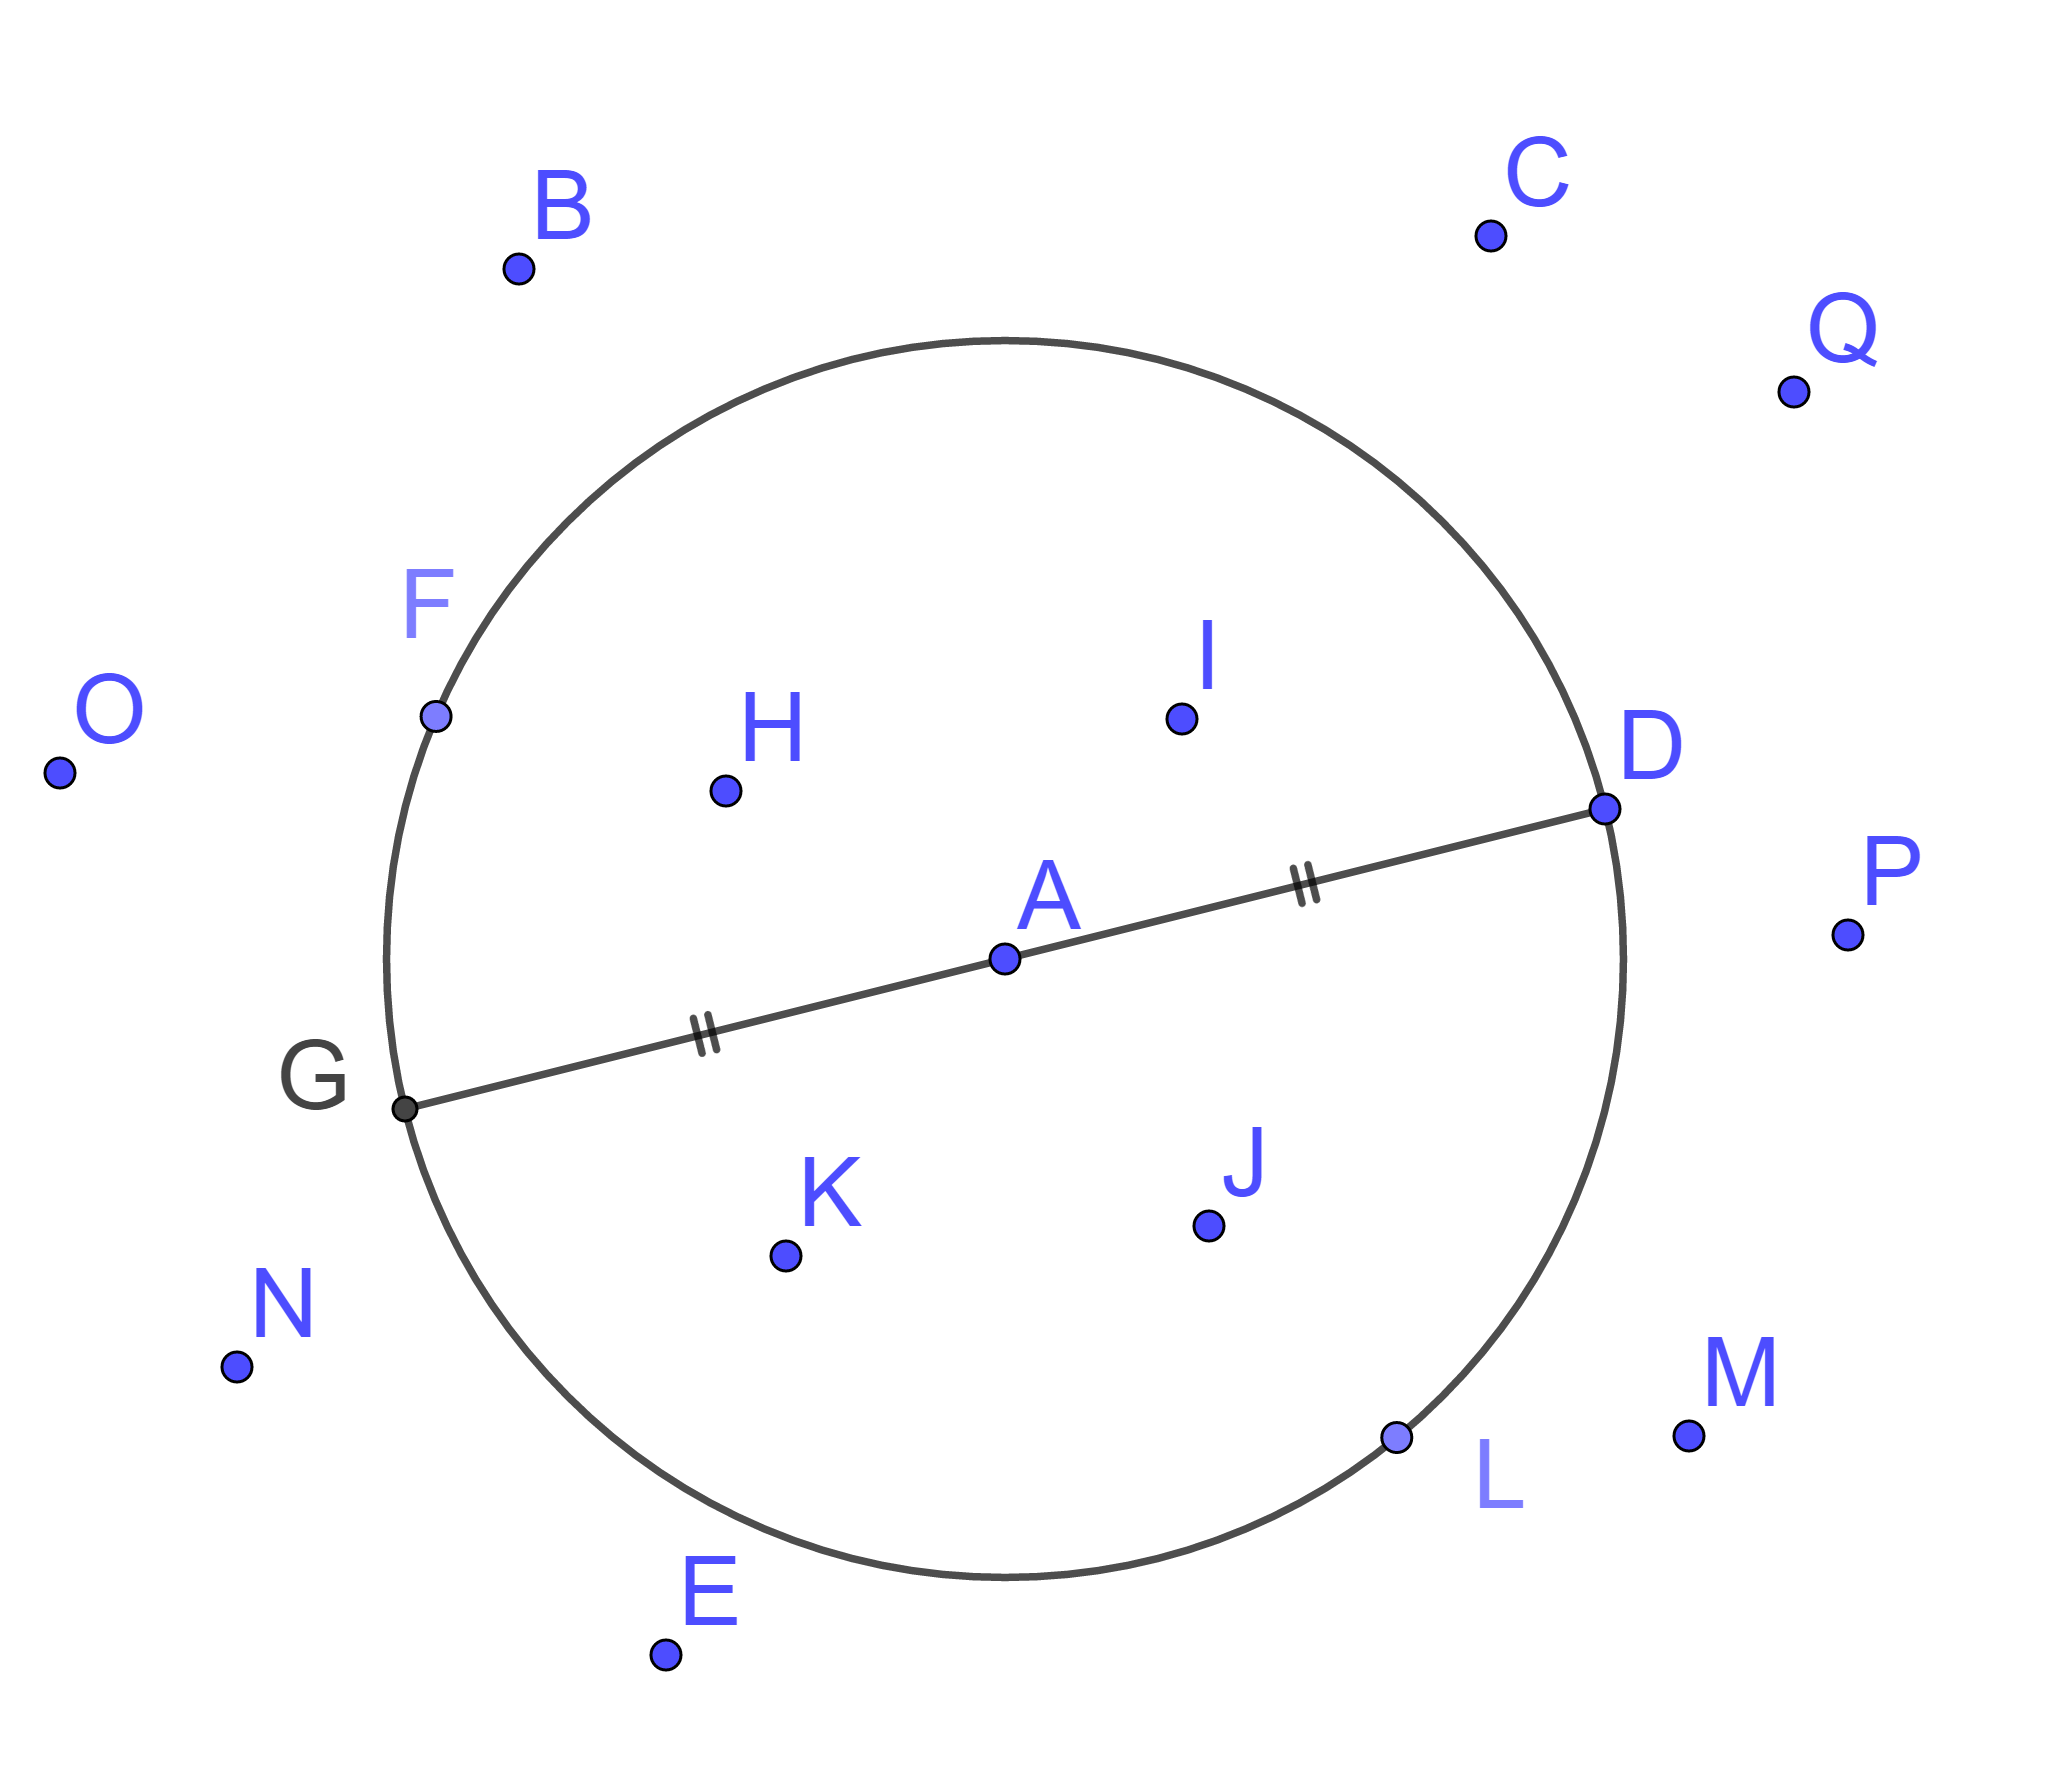
\includegraphics[scale=0.15]{./img/cercle}
\end{center}

\begin{questions}
	\question Pour ce cercle , citer :
	
	\begin{parts}
		\part[1] deux rayons;
		\part[\half] un diamètre.
	\end{parts}

	\question Citer tous les points situés à :
	
	\begin{parts}
		\part[\half] \num{2,7} cm du point A ;
		\part[\half] moins de \num{2,7} cm du point A;
		\part[\half] plus de \num{2,7} cm du point A;
	\end{parts}

	\question[1] Citer deux points situés à \num{5.4} cm l'un de l'autre.
\end{questions}